\subsubsection{Image Buffers}
\label{subsubsec:buffers}
% \todo[inline]{Citations}

Two different buffers with the same buffer size (\texttt{BS}) are used.
A Baumer image buffer to receive the images and an OpenCV matrix cirucular buffer to manipulate and save the images.

\paragraph{Baumer Image Buffer}
The received images are stored in Baumer \texttt{BGAPI2::Buffer} objects.
These are instantiated with the default constructor \texttt{BGAPI2::Buffer::Buffer()}, which allocates enough memory for the maximum payload of the camera.
In this case the maximum payload of the industrial camera is determined by the \texttt{BGR8} pixel format.
As a result of this, the memory utilization for the Baumer \texttt{BayerRG8} pixel format is only \SI{33}{\percent}.
Table \ref{tab:buffer_memory_utilization} shows the required memory as well as the memory utilization for the two pixel formats \texttt{BayerRG8} and \texttt{BGR8}.

\clearpage

It is possible to get \SI{100}{\percent} memory utilization with the Baumer \texttt{BayerRG8} pixel format.
The necessary memory for the specific payload size can be allocated manually and then passed to the constructor.
However, the software is not designed to run on an embedded system but on a computer.
Every modern computer should have the required resources to run the program.
% https://www.baumer.com/ch/en/product-overview/industrial-cameras-image-processing/software/baumer-gapi-sdk/c/14174

\begin{table}[t]
  \caption{Baumer image buffer memory utilization for the pixel formats \texttt{BayerRG8} and \texttt{BGR8}}
  \label{tab:buffer_memory_utilization}
  \centering
  \begin{tabular}{lll}
    \toprule
     & \textbf{\texttt{BayerRG8}} & \textbf{\texttt{BGR8}} \\
    \midrule
    \textbf{Bytes per pixel} & \SI{1}{B} & \SI{3}{B} \\
    \textbf{Pixel count} & \SI{1310720}{px} & \SI{1310720}{px} \\
    \textbf{Pixel bytes} & \SI{1310720}{B} & \SI{3932160}{B} \\
    \textbf{Buffer size} & \SI{3932160}{B} & \SI{3932160}{B} \\
    \textbf{Utilization} & \SI{33}{\percent} & \SI{100}{\percent} \\
    \bottomrule
  \end{tabular}
\end{table}

% --------------------------------
\paragraph{OpenCV Circular Buffer}
OpenCV matrix \texttt{cv::Mat} objects are used to perform the necessary image manipulations (see section \ref{subsubsec:image_change_detection}).
The data pointer of the Baumer image buffer is used to create an OpenCV matrix as shown in appendix \ref{app:throw_detection} on line \ref{lst:ln:buffer}.
This way, the OpenCV matrix does not allocate memory for the matrix data and uses the specified data.
The reasons for only creating such a shallow copy are efficiency and memory space.
% https://docs.opencv.org/4.1.1/d3/d63/classcv_1_1Mat.html#a51615ebf17a64c968df0bf49b4de6a3a

In order to be able to save the images later, past OpenCV matrices must be available.
For this reason, an OpenCV matrix circular buffer is used to keep track of them.
The structure of the circular buffer is shown in figure \ref{fig:circular_buffer}.
The circular buffer size (\texttt{BS}) is the same as the Baumer image buffer size.
The elements of the circular buffer can be accessed through an index $I$.
This index $I$ depends on the frame id (\texttt{FID}) and is calculated using equation \ref{eq:indexing}.

\begin{equation}
  I \equiv \text{FID} \pmod{\text{BS}}
  \label{eq:indexing}
\end{equation}

\begin{figure}[hb]
  \centering
  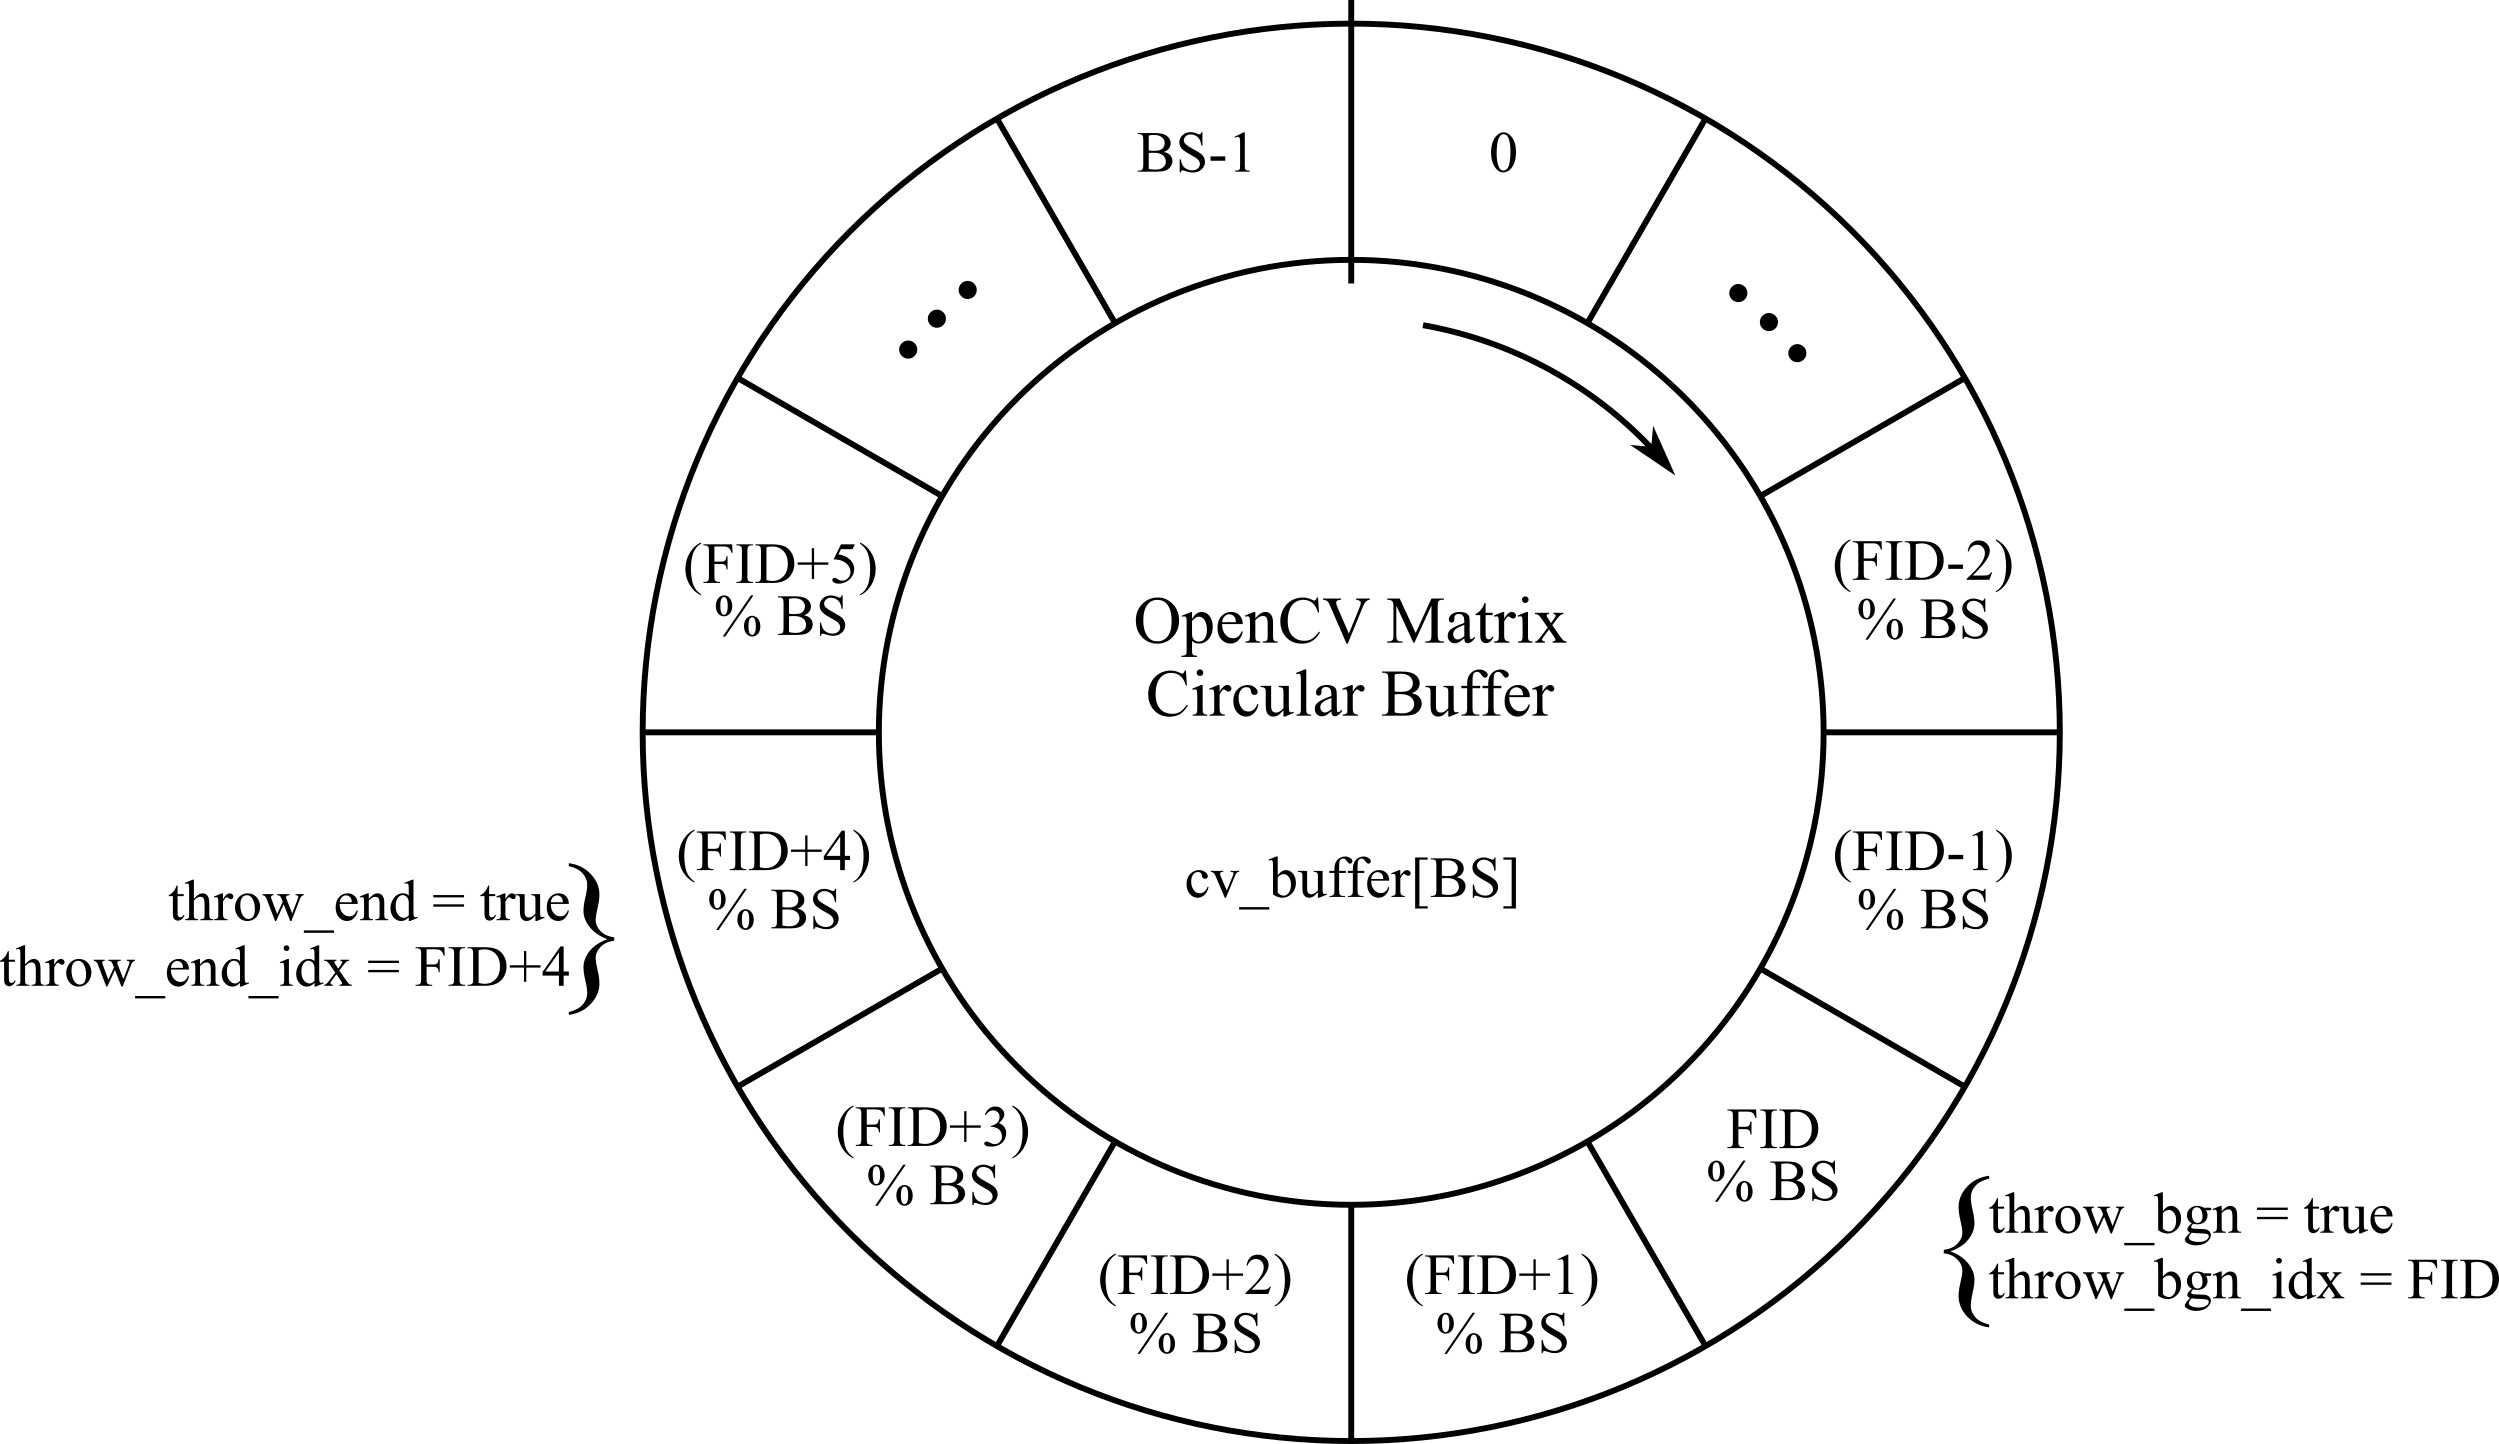
\includegraphics[width=0.9\textwidth]{buffer}
  \caption{OpenCV matrix circular buffer}
  \label{fig:circular_buffer}
\end{figure}
